\section{对角化与动力系统：把耦合演化变成独立缩放}
\label{sec:03-Linear-Algebra/05-Eigenvalues-and-Eigenvectors/02}

上一节找到了一些不转向的方向，但那还只是关于个别向量的话。真正想回答的问题是任意起点的长期去向：给定 \(x_0\) 与 \(A\)，\(x_k=A^kx_0\) 走到很远之后是什么样子。

只要 \(x_0\) 恰好是特征向量，答案立刻就有：\(A^kx_0=\lambda^kx_0\)。麻烦的是 \(x_0\) 一般不是。那就把它拆开——如果特征向量多到能张成整个空间，任何 \(x_0\) 都可以写成它们的组合，而每个组合分量各走各的，互不干扰。整节的技术内容不过是把这句话写成矩阵。

\subsection{把特征向量摆成一组基}

设 \(n\times n\) 矩阵 \(A\) 有 \(n\) 个线性无关的特征向量 \(v_1,\dots,v_n\)，对应特征值 \(\lambda_1,\dots,\lambda_n\)。把它们并成矩阵的列，特征值放到对角线上：

\[
S=\begin{pmatrix}v_1&\cdots&v_n\end{pmatrix},
\qquad
\Lambda=\diag(\lambda_1,\dots,\lambda_n).
\]

\(n\) 条关系 \(Av_i=\lambda_i v_i\) 合起来正是一次矩阵乘法 \(AS=S\Lambda\)。列独立意味着 \(S\) 可逆，于是

\[
S^{-1}AS=\Lambda,
\qquad
A=S\Lambda S^{-1}.
\]

这称为对角化。\(S\) 把特征坐标翻译成标准坐标，\(A\) 在标准坐标里干活，\(S^{-1}\) 再翻译回来；三步合起来，在特征坐标中看到的就是一个对角矩阵。变换本身一点没变，换的是记录它的基。

好处在乘幂时兑现。相邻的 \(S^{-1}S\) 逐对抵消，

\[
A^k=(S\Lambda S^{-1})^k=S\Lambda^kS^{-1},
\qquad
\Lambda^k=\diag(\lambda_1^k,\dots,\lambda_n^k).
\]

一个原本需要 \(k\) 次矩阵乘法的对象，塌成了 \(n\) 个标量的 \(k\) 次方。把 \(x_0\) 在特征基下展开成 \(x_0=c_1v_1+\cdots+c_nv_n\)，就得到这一节最该记住的式子：

\[
x_k=c_1\lambda_1^k v_1+\cdots+c_n\lambda_n^k v_n .
\]

耦合的演化被拆成 \(n\) 条独立的指数轨道，每条只由一个数控制。

\subsection{最大模特征值最终说了算}

上式里各项以不同速度变化。把特征值按模从大到小排，只要 \(\abs{\lambda_1}>\abs{\lambda_2}\) 且 \(c_1\neq 0\)，提出主项

\[
x_k=\lambda_1^k\Bigl(c_1v_1+\sum_{i\ge 2}c_i\Bigl(\frac{\lambda_i}{\lambda_1}\Bigr)^{k}v_i\Bigr),
\]

括号里除首项外每一项都带一个模小于 \(1\) 的数的 \(k\) 次方，按几何速率退场。方向上，\(x_k\) 被越拽越靠近 \(v_1\)。

\begin{center}
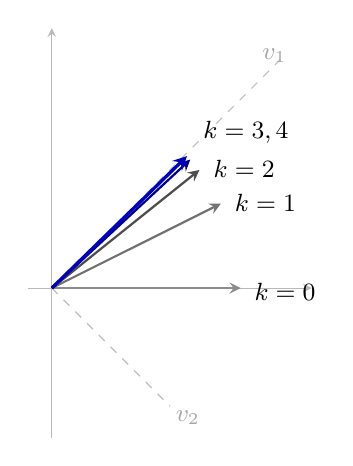
\begin{tikzpicture}[x=1cm,y=1cm,>=stealth]
  \draw[->,gray!55] (-0.3,0) -- (3.3,0);
  \draw[->,gray!55] (0,-1.9) -- (0,3.3);
  \draw[gray!50,dashed] (0,0) -- (2.9,2.9);
  \node[right,gray!70,font=\small] at (2.55,2.95) {\(v_1\)};
  \draw[gray!50,dashed] (0,0) -- (1.5,-1.5);
  \node[right,gray!70,font=\small] at (1.45,-1.65) {\(v_2\)};
  \draw[->,black!45,thick] (0,0) -- (2.4,0);
  \draw[->,black!55,thick] (0,0) -- (2.147,1.073);
  \draw[->,black!70,thick] (0,0) -- (1.874,1.500);
  \draw[->,blue!55!black,thick] (0,0) -- (1.758,1.632);
  \draw[->,blue!75!black,very thick] (0,0) -- (1.717,1.676);
  \node[right,font=\small] at (2.45,-0.05) {\(k=0\)};
  \node[right,font=\small] at (2.2,1.08) {\(k=1\)};
  \node[right,font=\small] at (1.93,1.52) {\(k=2\)};
  \node[right,font=\small] at (1.8,1.98) {\(k=3,4\)};
\end{tikzpicture}

\emph{把 \(x_k=A^kx_0\) 每步都归一化后画出来。方向从 \(x_0\) 出发一路向 \(v_1\) 靠拢，第四步已经几乎贴上去；沿 \(v_2\) 的那部分按 \((\lambda_2/\lambda_1)^k\) 消失。}
\end{center}

图里那条向 \(v_1\) 收拢的折线就是幂迭代的全部原理：反复乘 \(A\) 再归一化，就能逼近主特征方向，连特征多项式都不用写。收敛快慢由比值 \(\abs{\lambda_2/\lambda_1}\) 决定，这个比值离 \(1\) 越远收敛越快；两个模接近时，方向长时间在两条轴之间徘徊，算法迟迟定不下来。

同一件事在概率里有个熟面孔。转移矩阵作用在分布上时最大的特征值恒等于 \(1\)，对应的特征向量就是平稳分布——这正是它``乘上去不动''的含义；第二大模 \(\abs{\lambda_2}\) 与 \(1\) 的差距称为谱间隙，它决定链从任意初始分布收敛到平稳分布有多快。\hyperref[sec:06-Random-Processes/03-Markov-Chains/04]{``平稳分布、可逆性与遍历收敛''}会从概率一侧重讲这件事。PageRank 也是同一台机器：把网页的重要性向量反复沿链接分发，收敛到的就是主特征向量，工程上加的阻尼因子正是为了压住 \(\abs{\lambda_2}\)、保证间隙不消失。

\subsection{模与 \texorpdfstring{\(1\)}{1} 的关系划出三种命运}

离散系统 \(x_{k+1}=Ax_k\) 的长期行为，逐模式地由 \(\abs{\lambda_i}\) 落在 \(1\) 的哪一侧决定。

\begin{center}
\begin{tikzpicture}[x=1cm,y=0.62cm,font=\small]
  \begin{scope}
    \draw[gray!55,->] (-0.2,0) -- (2.3,0);
    \draw[gray!35,dashed] (-0.2,1) -- (2.3,1);
    \foreach \k in {0,1,2,3,4,5}
      \fill[blue!65!black] (0.35*\k,{pow(0.62,\k)}) circle (2pt);
    \node at (1.05,-1.05) {\(\abs{\lambda}<1\)};
    \node at (1.05,-2.0) {衰减到零};
  \end{scope}
  \begin{scope}[shift={(3.4,0)}]
    \draw[gray!55,->] (-0.2,0) -- (2.3,0);
    \draw[gray!35,dashed] (-0.2,1) -- (2.3,1);
    \foreach \k in {0,1,2,3,4,5}
      \fill[blue!65!black] (0.35*\k,1) circle (2pt);
    \node at (1.05,-1.05) {\(\abs{\lambda}=1\)};
    \node at (1.05,-2.0) {临界，需另行判断};
  \end{scope}
  \begin{scope}[shift={(6.8,0)}]
    \draw[gray!55,->] (-0.2,0) -- (2.3,0);
    \draw[gray!35,dashed] (-0.2,1) -- (2.3,1);
    \foreach \k in {0,1,2,3,4,5}
      \fill[blue!65!black] (0.35*\k,{pow(1.28,\k)}) circle (2pt);
    \node at (1.05,-1.05) {\(\abs{\lambda}>1\)};
    \node at (1.05,-2.0) {指数发散};
  \end{scope}
\end{tikzpicture}

\emph{同一条特征方向上分量的模随步数的变化。虚线是初始高度，三种情形只差 \(\abs{\lambda}\) 与 \(1\) 的相对位置；中间那种最脆弱，下一节会给出特征值全在单位圆上却仍然发散的矩阵。}
\end{center}

最大模

\[
\rho(A)=\max_i\abs{\lambda_i}
\]

称为谱半径。\(\rho(A)<1\) 时所有模式衰减，系统渐近稳定；\(\rho(A)>1\) 时至少一条方向在放大，系统发散。恰好等于 \(1\) 的情形不能只看特征值，还要看特征方向够不够——这是下一节的主题。

深度学习里对这三种命运的感受最直接。循环网络反向传播时，梯度要连乘许多步的 Jacobi 矩阵；若这些矩阵近似同一个 \(A\)，梯度大小就按 \(\rho(A)^k\) 走。谱半径小于 \(1\)，几十步之后梯度衰减到浮点数分辨不出，远处的依赖学不到，这是梯度消失；大于 \(1\) 则连乘迅速溢出，是梯度爆炸。正交或近似正交的循环权重初始化，用意就是把谱半径按住在 \(1\) 附近；梯度裁剪则是对爆炸一侧的事后补救。\hyperref[sec:14-Deep-Learning/03-Optimization-and-Training/01]{``训练动力学与数值稳定''}会把这些手段放在一起比较。

优化里出现的是另一种读法。梯度下降在极小点附近的误差满足 \(e_{k+1}\approx(I-\eta H)e_k\)，\(H\) 是 Hessian 矩阵。这个迭代矩阵的特征值是 \(1-\eta\mu_i\)，其中 \(\mu_i\) 是 Hessian 的特征值，也就是各方向上的曲率。步长 \(\eta\) 必须让所有 \(\abs{1-\eta\mu_i}<1\)，于是同时受最大曲率与最小曲率的挤压，可用的收敛速率被条件数 \(\mu_{\max}/\mu_{\min}\) 卡住。曲率谱因此不是一个抽象的量，它直接换算成``要跑多少步''，\hyperref[sec:09-Convex-Optimization/06-Optimization-Algorithms/01]{``梯度下降真正难在步长''}正是围绕这一点展开。

\subsection{连续时间换一套判据}

把步进换成微分方程 \(\dot x=Ax\)，解是 \(x(t)=e^{At}x(0)\)，其中矩阵指数由幂级数定义：

\[
e^{At}=\sum_{k=0}^{\infty}\frac{t^k}{k!}A^k .
\]

逐项求导给出 \(\tfrac{d}{dt}e^{At}=Ae^{At}\)，代入 \(t=0\) 得单位矩阵，方程与初值都对得上。把 \(A^k=S\Lambda^kS^{-1}\) 代进去，每一项都提着同一对 \(S\) 和 \(S^{-1}\)，于是

\[
e^{At}=S\,e^{\Lambda t}\,S^{-1},
\qquad
e^{\Lambda t}=\diag(e^{\lambda_1t},\dots,e^{\lambda_nt}),
\]

对应的解是 \(x(t)=\sum_i c_ie^{\lambda_it}v_i\)。判据随之改变：连续时间看的是实部，\(\operatorname{Re}\lambda_i<0\) 给出衰减，大于零给出发散；虚部只管转，\(e^{(a+bi)t}=e^{at}(\cos bt+i\sin bt)\) 里 \(a\) 定包络、\(b\) 定频率。

两套判据不能混用。离散比 \(\abs{\lambda}\) 与 \(1\)，连续比 \(\operatorname{Re}\lambda\) 与 \(0\)；把其中一条套到另一种系统上，稳定与发散的结论会整个翻转。记混时可以回到 \(\lambda^k\) 与 \(e^{\lambda t}\) 这两个原型，一个是乘幂，一个是指数，谁该跟谁比一目了然。控制理论把左半平面称作稳定区、把单位圆内称作稳定区，用的就是这两条线；\hyperref[sec:16-Control-and-Reinforcement-Learning/01-Optimal-Control/01]{``从开环到闭环反馈''}讨论的反馈设计，说到底是用 \(u=-Kx\) 把闭环矩阵 \(A-BK\) 的特征值搬到稳定区里去。

\subsection{什么时候凑不齐一组基}

\(A\) 可对角化，当且仅当它拥有 \(n\) 个线性无关的特征向量，也就是各特征空间维数之和等于 \(n\)。上一节给过一个方便的充分条件：\(n\) 个互不相同的特征值。它不必要——单位矩阵只有一个特征值却毫无障碍地对角化，因为它的特征空间就是全空间。

失败只有一种方式：某个特征值的几何重数严格小于代数重数。最小的例子仍是

\[
J=\begin{pmatrix}0&1\\0&0\end{pmatrix},
\]

特征值 \(0\) 重数为 \(2\)，特征向量却只有 \((c,0)^{\trans}\) 这一条线。缺了一条方向，就没有一组特征向量能张成 \(\R^2\)，\(S\) 也就拼不出来。下一节会说明这种缺陷带来的不是``算不了''，而是一种新的增长方式。

\subsection{对称矩阵才有正交的特征基}

一般可对角化矩阵写成 \(A=S\Lambda S^{-1}\)，\(S\) 的列没有任何理由彼此垂直。当特征方向接近平行时 \(S\) 病态，\(S^{-1}\) 的元素巨大，数值上这个分解就靠不住了。

实对称矩阵是例外。它总能写成

\[
A=Q\Lambda Q^{\trans},
\]

其中 \(Q\) 正交、\(\Lambda\) 实对角。逆就是转置，特征方向互相垂直，分解在数值上稳定得多。这条结论叫谱定理，\hyperref[sec:03-Linear-Algebra/06-Symmetric-and-Positive-Definite-Matrices/01]{``对称矩阵与谱定理：什么时候特征方向一定正交''}会给出它成立的理由。协方差矩阵、Hessian 矩阵、图的 Laplace 矩阵都对称，实践中遇到的谱分解多半属于这一类，这也是为什么许多人对特征分解的第一印象是``特征向量总是正交的''。

那种印象在一般矩阵上会立刻出错。看到 \(A=S\Lambda S^{-1}\) 就顺手把 \(S^{-1}\) 写成 \(S^{\trans}\) 是本章最常见的失误，只有确认了对称性才允许这么做。

到这里，能对角化的情形已经交代完：换到特征基，重复作用就是几个标量各自取幂，长期行为由最大模那个说了算。下一节把这个前提拿掉，看看方向不够用时，缺掉的那一维会以什么形式在解里重新冒出来。
